\documentclass[a4paper,10pt]{article}
\usepackage[paperwidth=210mm, paperheight=297mm, left=2.5cm, top=2.5cm, right=2.5cm, bottom=1.0cm, head=1.5cm, includefoot]{geometry}
%\usepackage[latin1]{inputenc}

\usepackage[english]{babel}
\usepackage[utf8x]{inputenc}
\usepackage{amsmath}

\usepackage{bookman}
\usepackage{booktabs}
\usepackage[pdfborder={0 0 0}]{hyperref}
\usepackage{pdfpages}
\usepackage{fancyhdr}
\usepackage{lastpage}
\usepackage{verbatim}
\usepackage{graphicx}
\usepackage{fixltx2e}
\usepackage{listings}

%\usepackage[T1]{fontenc}
%\usepackage{comment}
%\usepackage{makeidx}
%\usepackage{float}
%\usepackage{slashbox}

\renewcommand{\headrulewidth}{1pt}
\renewcommand{\footrulewidth}{1pt}



%%%%%%%%%  Datos  %%%%%%%%%

\title{ \textbf{Trabajo práctico 1: Conjunto de instrucciones MIPS} }

\author{Contini, Agustín - \textit{Padrón 89180}			\\
            \texttt{ agscontini@gmail.com }				\\
            Farina, Federico - \textit{Padrón 90177}			\\
            \texttt{ federicojosefarina@gmail.com }				\\
            Prystupiuk, Maximiliano  - \textit{Padrón 94853  }			\\
            \texttt{ mprystupiuk@gmail.com  }					\\[2.5ex]
            1er. Cuatrimestre de 2017					\\[1.0ex]
            \normalsize{66.20 Organización de Computadoras}		\\
            \normalsize{Facultad de Ingeniería, Universidad de Buenos Aires}	\\
	}
\date{\today}

%%%%%%%%%  Fin datos  %%%%%%%%%



\begin{document}



%%%%%%%%%  1era hoja: caratula y datos  %%%%%%%%%

\maketitle
\bigskip
\thispagestyle{empty}	% quita el numero en la primera pagina

\begin{abstract}
El trabajo consiste conseguir que un conjunto de programas
cumplan con una condición, cuando normalmente no lo harían, aprovechando las vulnerabilidades del stack y de la función gets() teniendo un buffer de largo fijo y conocido.
Para este cometido se utilizará gdb y objdump como herramientas sobre MIPS32 en un entorno NetBSD.

\end{abstract}



%%%%%%%%%  Fin 1era hoja  %%%%%%%%%



%%%%%%%%%  Head y foot  %%%%%%%%%

\pagestyle{fancy}
\lhead{
\includegraphics[width=1.2cm]{./img/logo.png}}
\chead{Trabajo práctico 1: Conjunto de instrucciones MIPS \\ \textit{Contini  -  Farina  -  Prystupiuk} }

\rfoot{$1^{er}$ Cuatrimestre 2017}
\lfoot{66.20 Organizaci\'on de Computadoras}
\cfoot{\hspace{2.4cm}   P\'agina \thepage \, de \pageref{LastPage} }

%%%%%%%%%  Fin head y foot  %%%%%%%%%



\normalsize

\newpage
\tableofcontents	% hoja de indices de titulos, subtitulos

\vspace{2.0cm}
\listoffigures		% hoja de indices de figuras

\newpage
\section{Introducci\'on}

\subsection{Problemas de programación insegura}

Los ejercicios a analizar fueron diseñados especialmente para la compresión del funcionamiento de los programas compilados en C por Gerardo Richarte y son de especial interés para la compresión del stack y la explotación de sus vulnerabilidades.
\par El trabajo consiste en conseguir que los programas stack1.c a stack5.c cumplan una condición y impriman la frase "you win!" aprovechando que utilizan la función gets para llenar un buffer de largo fijo y conocido utilizando gdb para examinar el stack y los valores de los registros y objdump para inspeccionar de manera sencilla las posiciones relativas al stack pointer.


\newpage
\section{Uso}
\subsection{Compilado}
Dentro del entorno de NetBSD, en el directorio del proyecto ejecutar para cada archivo i:

\begin{verbatim}
$ gcc -g stack{i}.c -o stack{i}.o
\end{verbatim}

\subsection{Herramientas utilizadas}
\subsubsection{GDB}

Poner alguna fruta:

\begin{verbatim}
$ gdb stack1.o
\end{verbatim}

\subsubsection{Objdump}

Alguna fruta más:

\begin{verbatim}
$ objdump -d stack{i}.o
\end{verbatim}

\newpage
\section{Programas}
\subsection{stack1}
\lstset{ language = C, numbers=left, tabsize=4, breaklines=true, frame=single }
\lstinputlisting{./stack1.c}

\bigskip
El buffer ocupa el espacio de 80 char, lo que corresponde a 20 words en el stack que se corresponden con el rango [24(sp), 103(sp)]

Al ser \textbf{fgets()} una función insegura y estando cookie y más fruta...

\bigskip

\begin{figure}[h!]
	\centering
	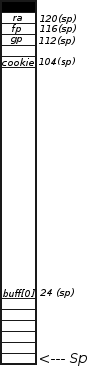
\includegraphics[scale=0.7]{./recursos/stack1.png}
	\caption{Gr\'afico del speedup entre Bubblsort en C y Quicksort en C}
\end{figure}





\subsection{stack2}
\lstset{ language = C, numbers=left, tabsize=4, breaklines=true, frame=single }
\lstinputlisting{./stack2.c}

\subsection{stack3}
\lstset{ language = C, numbers=left, tabsize=4, breaklines=true, frame=single }
\lstinputlisting{./stack3.c}

\subsection{stack4}
\lstset{ language = C, numbers=left, tabsize=4, breaklines=true, frame=single }
\lstinputlisting{./stack4.c}

\subsection{stack5}

\lstset{ language = C, numbers=left, tabsize=4, breaklines=true, frame=single }
\lstinputlisting{./stack5.c}

\lstset{ language = C, numbers=left, tabsize=4, breaklines=true, frame=single }
\lstinputlisting{./stack5.h}

\lstset{ language = C, numbers=left, tabsize=4, breaklines=true, frame=single }
\lstinputlisting{./win.h}

\lstset{ language = C, numbers=left, tabsize=4, breaklines=true, frame=single }
\lstinputlisting{./win.c}









\end{document}
